\documentclass{beamer}[12pt]
\usetheme{boxes}
\usecolortheme{seahorse}
\beamertemplatenavigationsymbolsempty
\setbeamertemplate{items}[triangle]
\usepackage{tikz}
\usepackage{tkz-graph}
\usepackage{pgfplots} 
\usepackage{xcolor}
\usepackage{amsmath}
\usepackage{amsthm}

\author{Fynn Lohren, Leon Suchy, Carsten Schubert}
\date{\today}
\title{Presentation 5}

\begin{document}
	\frame{\titlepage}
	
	\begin{frame}
		\frametitle{Structure}
		\begin{itemize}
			\item Optimization
			\item Data Reductions
			\item Lower Bounds
			\item Configurations
			\item SMAC
			\item Overview
			\item Conclusion
		\end{itemize}
	\end{frame}
	
	\begin{frame}
		\frametitle{Lower Bounds - Clique Cover}
		Improvement Idea: \\ \vspace{3mm}
		
		Try to improve solution \\
		$\rightarrow$ combine cliques of small size to cycles or cliques \\
		$\rightarrow$ failed to improve solution most of the time
	\end{frame}	
	
	\begin{frame}
		\frametitle{Lower Bounds - Cycle Cover}
		
		Compute Cycle Cover from matching in LP-Graph:
		
		\vspace{7mm}
		\pause
		
		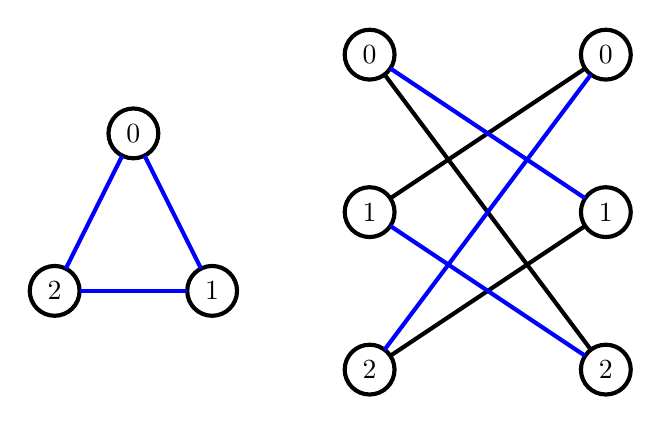
\begin{tikzpicture}
			%\draw[help lines] (0,0) grid (10,6);
			
			\SetVertexNormal[Shape = circle, LineWidth = 1.5pt]
			\SetUpEdge[lw = 1.5pt, color = black]
			
			\Vertex[x=2,y=4,L=$0$]{0}
			\Vertex[x=3,y=2,L=$1$]{1}	
			\Vertex[x=1,y=2,L=$2$]{2}
			
			\Vertex[x=5,y=5,L=$0$]{10}
			\Vertex[x=5,y=3,L=$1$]{11}	
			\Vertex[x=5,y=1,L=$2$]{12}
			
			\Vertex[x=8,y=5,L=$0$]{20}
			\Vertex[x=8,y=3,L=$1$]{21}	
			\Vertex[x=8,y=1,L=$2$]{22}
			
			\Edges(10,22)
			\Edges(11,20)
			\Edges(12,21)
			\SetUpEdge[
			lw 		= 1.5pt,
			color 	= blue]
			
			\Edges(10, 21)
			\Edges(11, 22)
			\Edges(12, 20)
			
			\Edges(0,1,2,0)
		\end{tikzpicture}
	\end{frame}

	\begin{frame}
		\frametitle{Lower Bounds - Cycle Cover}
		
		\begin{itemize}
			\item After LP-Reduction perfect matching
			\item Take corresponding edge in original graph for each edge in matching
			\item When LP-Reduction not applied we just build our cycle incrementally
		\end{itemize}
		
		\pause 
		
		\begin{itemize}
			\item Did not make it into final solver
			\item LP-Reduction and Hopcroft-Karp too slow
			\item Noticed too late
		\end{itemize}
	\end{frame}

	\begin{frame}
		\frametitle{Testinstances}
		
		\begin{itemize}
			\item 47 Instances
			\item Instances that were hard for handpicked
			\item Nearly solved by handpicked
		\end{itemize}
	\end{frame}
	
	\begin{frame}
	\frametitle{SMAC Run 1}
	
	\begin{tikzpicture}
	\begin{axis}
	[
	width=0.9\textwidth,
	height=0.5\textwidth,
	xlabel={k},
	ylabel={time},
	legend cell align=left,
	legend pos=south east,
	legend entries={dimacs, pace, snap},
	legend style={at={(1.22,0.645), anchor=north, columns=-1}}
	]
	
	\addplot[only marks,color=black, mark=triangle*] table[col sep=comma,y={Time}, x={VC}] {smac_new_dimacs.csv};
	\addplot[only marks,color=red, mark=triangle*] table[col sep=comma,y={Time}, x={VC}] {smac_new_pace.csv};
	\addplot[only marks,color=blue, mark=triangle*] table[col sep=comma,y={Time}, x={VC}] {smac_new_snap.csv};
	\end{axis}
	\end{tikzpicture}
	\end{frame}

	\begin{frame}
		\frametitle{SMAC Run 2}
		
		\begin{tikzpicture}
			\begin{axis}
			[
			width=0.9\textwidth,
			height=0.5\textwidth,
			xlabel={k},
			ylabel={time},
			legend cell align=left,
			legend pos=south east,
			legend entries={dimacs, pace, snap},
			legend style={at={(1.22,0.645), anchor=north, columns=-1}}
			]
			
			\addplot[only marks,color=black, mark=triangle*] table[col sep=comma,y={Time}, x={VC}] {smac_dimacs.csv};
			\addplot[only marks,color=red, mark=triangle*] table[col sep=comma,y={Time}, x={VC}] {smac_pace.csv};
			\addplot[only marks,color=blue, mark=triangle*] table[col sep=comma,y={Time}, x={VC}] {smac_snap.csv};
			\end{axis}
		\end{tikzpicture}
	\end{frame}
	
	\begin{frame}
		\frametitle{Handpicked}
		
		\begin{tikzpicture}
		\begin{axis}
		[
		width=0.9\textwidth,
		height=0.5\textwidth,
		xlabel={k},
		ylabel={time},
		legend cell align=left,
		legend pos=south east,
		legend entries={dimacs, pace, snap},
		legend style={at={(1.22,0.645), anchor=north, columns=-1}}
		]
		
		\addplot[only marks,color=black, mark=triangle*] table[col sep=comma,y={Time}, x={VC}] {handpicked_dimacs.csv};
		\addplot[only marks,color=red, mark=triangle*] table[col sep=comma,y={Time}, x={VC}] {handpicked_pace.csv};
		\addplot[only marks,color=blue, mark=triangle*] table[col sep=comma,y={Time}, x={VC}] {handpicked_snap.csv};
		\end{axis}
		\end{tikzpicture}
	\end{frame}
	
	
	\begin{frame}
		\frametitle{Recursive Steps}
		\begin{tikzpicture}
			\begin{loglogaxis}[
			width=0.9\textwidth,
			height=0.5\textwidth,
			xlabel={Handpicked},
			ylabel={SMAC},
			legend cell align=left,
			legend pos=south east,
			legend entries={dimacs, pace, snap},
			legend style={at={(1.22,0.645), anchor=north, columns=-1}},
			ymode=log,
			xmin=0.5,
			ymin=0.5,
			xmax=100000,
			ymax=100000,
			]
			
			\addplot[only marks,color=black, mark=triangle*] table[col sep=comma,y={SMAC}, x={Ours}] {smac_ours_comparison_dimacs.csv};
			
			\addplot[only marks,color=red, mark=triangle*] table[col sep=comma,y={SMAC}, x={Ours}] {smac_ours_comparison_pace.csv};
			
			\addplot[only marks,color=blue, mark=triangle*] table[col sep=comma,y={SMAC}, x={Ours}] {smac_ours_comparison_snap.csv};
			
			\addplot[color=black,domain=0.5:100000,samples=4] {x};
			\end{loglogaxis}
		\end{tikzpicture}
	\end{frame}

	\begin{frame}
		\frametitle{Execution Time}
		\begin{tikzpicture}
		\begin{loglogaxis}[
		width=0.9\textwidth,
		height=0.5\textwidth,
		xlabel={Handpicked},
		ylabel={SMAC},
		legend cell align=left,
		legend pos=south east,
		legend entries={dimacs, pace, snap},
		legend style={at={(1.22,0.645), anchor=north, columns=-1}},
		ymode=log,
		xmin=0.005,
		ymin=0.005,
		xmax=500,
		ymax=500,
		]
		
		\addplot[only marks,color=black, mark=triangle*] table[col sep=comma,y={TSMAC}, x={TOurs}] {smac_ours_comparison_dimacs.csv};
		
		\addplot[only marks,color=red, mark=triangle*] table[col sep=comma,y={TSMAC}, x={TOurs}] {smac_ours_comparison_pace.csv};
		
		\addplot[only marks,color=blue, mark=triangle*] table[col sep=comma,y={TSMAC}, x={TOurs}] {smac_ours_comparison_snap.csv};
		
		\addplot[color=black,domain=0.005:500,samples=4] {x};
		\end{loglogaxis}
	\end{tikzpicture}
\end{frame}
\end{document}

